\documentclass[11pt, a4paper]{article}

% Fonts and Encoding
\usepackage[utf8]{inputenc}
\usepackage[T1]{fontenc}
\usepackage{lmodern}
% Math and Symbols
\usepackage{amsmath, amssymb, amsthm, amsfonts, mathrsfs, mathtools}

% Layout and Geometry
\usepackage{geometry}
\geometry{a4paper, margin=1in}

% Formatting and Graphics
\usepackage{graphicx, xcolor, enumitem, booktabs, array, tabularx}

% TikZ for Illustrations
\usepackage{tikz}
\usetikzlibrary{arrows.meta, positioning, shapes.geometric, calc, backgrounds, matrix}

% Clickable Links and TOC
\usepackage{hyperref}
\hypersetup{
    colorlinks=true,
    linkcolor=blue,
    filecolor=magenta,      
    urlcolor=cyan,
    pdftitle={Advanced Mathematics Topic: Diagonalization},
}

% Theorem Environments
\newtheorem{theorem}{Theorem}[section]
\newtheorem{lemma}[theorem]{Lemma}
\newtheorem{proposition}[theorem]{Proposition}
\newtheorem{corollary}[theorem]{Corollary}
\theoremstyle{definition}
\newtheorem{definition}{Definition}[section]
\newtheorem{axiom}{Axiom}[section]
\newtheorem{example}{Example}[section]
\theoremstyle{remark}
\newtheorem{remark}{Remark}[section]

% Custom Commands (Enforced standard notation)
\newcommand{\R}{\mathbb{R}}
\newcommand{\N}{\mathbb{N}}
\newcommand{\Z}{\mathbb{Z}}
\newcommand{\Q}{\mathbb{Q}}
\newcommand{\E}{\mathbb{E}}
\newcommand{\Prob}{\mathbb{P}}
\newcommand{\F}{\mathcal{F}}

\title{\textbf{Mastering Linear Algebra: Diagonalization}}
\author{Tashfeen Omran}
\date{\today}

\begin{document}

\maketitle
\tableofcontents
\newpage

\section{Part 1: Comprehensive Introduction, Context, and Prerequisites}

\subsection{Core Concepts}
Diagonalization is a profound concept in linear algebra that simplifies the action of a square matrix by finding a special coordinate system (a basis) in which the matrix acts purely by scaling. If a matrix $A$ is diagonalizable, it can be factored into the form $A = PDP^{-1}$, where $D$ is a diagonal matrix containing the eigenvalues of $A$, and $P$ is an invertible matrix whose columns are the corresponding eigenvectors. 

In this new basis defined by $P$, the linear transformation represented by $A$ is completely decoupled. Instead of variables interacting with one another in complex ways, each variable simply scales independently by its respective eigenvalue.

\subsection{Intuition and Derivation}
Why do we care about the factorization $A = PDP^{-1}$? Consider the task of computing $A^k$ for some large integer $k$. Matrix multiplication is computationally expensive. However, if we can diagonalize $A$, we observe a beautiful telescoping cancellation:
\[
A^2 = (PDP^{-1})(PDP^{-1}) = PD(P^{-1}P)DP^{-1} = PDI DP^{-1} = PD^2P^{-1}
\]
By induction, this generalizes to $A^k = PD^kP^{-1}$. Because $D$ is diagonal, computing $D^k$ is trivial—we simply raise each diagonal entry to the $k$-th power. The matrices $P$ and $P^{-1}$ act as translators: $P^{-1}$ translates a vector into the ``eigenvector language,'' $D^k$ scales the vector effortlessly, and $P$ translates the result back to the standard basis.

\begin{center}
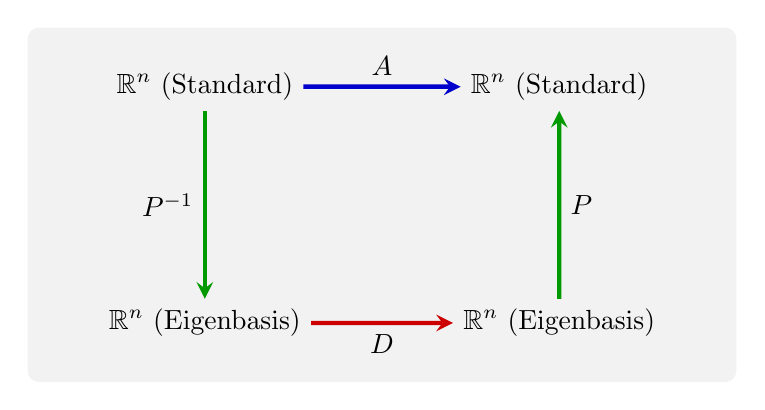
\begin{tikzpicture}[scale=1.5, >=stealth, thick]
    % Background
    \begin{scope}[on background layer]
        \fill[gray!10, rounded corners] (-1.5, -1.5) rectangle (4.5, 1.5);
    \end{scope}

    % Nodes
    \node[text=black] (V1) at (0, 1) {$\displaystyle \R^n \text{ (Standard)}$};
    \node[text=black] (V2) at (3, 1) {$\displaystyle \R^n \text{ (Standard)}$};
    \node[text=black] (W1) at (0, -1) {$\displaystyle \R^n \text{ (Eigenbasis)}$};
    \node[text=black] (W2) at (3, -1) {$\displaystyle \R^n \text{ (Eigenbasis)}$};

    % Arrows
    \draw[->, ultra thick, blue!80!black] (V1) -- (V2) node[midway, above, text=black] {$A$};
    \draw[->, ultra thick, red!80!black] (W1) -- (W2) node[midway, below, text=black] {$D$};
    \draw[->, ultra thick, green!60!black] (V1) -- (W1) node[midway, left, text=black] {$P^{-1}$};
    \draw[->, ultra thick, green!60!black] (W2) -- (V2) node[midway, right, text=black] {$P$};
\end{tikzpicture}
\end{center}

\subsection{Historical Context and Motivation}
The concept of eigenvalues and diagonalization emerged in the 19th century through the work of Augustin-Louis Cauchy, James Joseph Sylvester, and Arthur Cayley. The primary motivation was not abstract algebra, but rather the study of quadratic forms and celestial mechanics. Mathematicians needed to solve massive systems of linear differential equations to predict planetary orbits. By finding a basis of eigenvectors, they could ``uncouple'' these differential equations, turning a complex, interconnected system into a set of simple, independent equations that could be solved individually.

\subsection{Key Formulas}
\begin{itemize}
    \item \textbf{Diagonalization Factorization:} $A = PDP^{-1}$
    \item \textbf{Matrix Powers:} $A^k = PD^kP^{-1}$
    \item \textbf{Characteristic Equation:} $\det(A - \lambda I) = 0$ (used to find eigenvalues $\lambda$)
    \item \textbf{Eigenspace Nullity:} $\text{Nul}(A - \lambda I)$ (used to find eigenvectors)
\end{itemize}

\subsection{Prerequisites}
To master this topic, you must be fluent in:
\begin{enumerate}
    \item \textbf{Determinants:} Computing determinants of $2 \times 2$ and $3 \times 3$ matrices.
    \item \textbf{Null Spaces:} Using Gaussian elimination (row reduction) to find the basis of a null space.
    \item \textbf{Matrix Inversion:} Specifically, the formula for the inverse of a $2 \times 2$ matrix: 
    \[ \begin{bmatrix} a & b \\ c & d \end{bmatrix}^{-1} = \frac{1}{ad-bc} \begin{bmatrix} d & -b \\ -c & a \end{bmatrix} \]
\end{enumerate}

\newpage
\section{Part 2: Detailed Homework Solutions}
\textit{Note: Based on the strategic problem selection protocol, I have selected a representative sample of problems that cover every distinct archetype present in the provided text.}

\subsection{Problem 1 (Exercise 1)}
\textbf{Statement:} Compute $A^4$, where $P = \begin{bmatrix} 5 & 7 \\ 2 & 3 \end{bmatrix}$, $D = \begin{bmatrix} 2 & 0 \\ 0 & 1 \end{bmatrix}$, and $A = PDP^{-1}$.

\textbf{Solution:}
First, we must find $P^{-1}$. Using the $2 \times 2$ inverse formula:
\[
\det(P) = (5)(3) - (7)(2) = 15 - 14 = 1
\]
\[
P^{-1} = \frac{1}{1} \begin{bmatrix} 3 & -7 \\ -2 & 5 \end{bmatrix} = \begin{bmatrix} 3 & -7 \\ -2 & 5 \end{bmatrix}
\]
Next, we compute $D^4$. Since $D$ is diagonal, we simply raise the diagonal entries to the 4th power:
\[
D^4 = \begin{bmatrix} 2^4 & 0 \\ 0 & 1^4 \end{bmatrix} = \begin{bmatrix} 16 & 0 \\ 0 & 1 \end{bmatrix}
\]
Now, we use the property $A^4 = PD^4P^{-1}$. We compute this via two matrix multiplications. First, $PD^4$:
\[
PD^4 = \begin{bmatrix} 5 & 7 \\ 2 & 3 \end{bmatrix} \begin{bmatrix} 16 & 0 \\ 0 & 1 \end{bmatrix} = \begin{bmatrix} 5(16) + 7(0) & 5(0) + 7(1) \\ 2(16) + 3(0) & 2(0) + 3(1) \end{bmatrix} = \begin{bmatrix} 80 & 7 \\ 32 & 3 \end{bmatrix}
\]
Finally, we multiply by $P^{-1}$:
\[
A^4 = (PD^4)P^{-1} = \begin{bmatrix} 80 & 7 \\ 32 & 3 \end{bmatrix} \begin{bmatrix} 3 & -7 \\ -2 & 5 \end{bmatrix}
\]
\[
A^4 = \begin{bmatrix} 80(3) + 7(-2) & 80(-7) + 7(5) \\ 32(3) + 3(-2) & 32(-7) + 3(5) \end{bmatrix} = \begin{bmatrix} 240 - 14 & -560 + 35 \\ 96 - 6 & -224 + 15 \end{bmatrix} = \begin{bmatrix} 226 & -525 \\ 90 & -209 \end{bmatrix}
\]
\textbf{Final Answer:} $\displaystyle A^4 = \begin{bmatrix} 226 & -525 \\ 90 & -209 \end{bmatrix}$

\subsection{Problem 2 (Exercise 3)}
\textbf{Statement:} Use the factorization $A = PDP^{-1}$ to compute $A^k$, where $k$ represents an arbitrary positive integer.
\[
A = \begin{bmatrix} a & 0 \\ 3(a-b) & b \end{bmatrix} = \begin{bmatrix} 1 & 0 \\ 3 & 1 \end{bmatrix} \begin{bmatrix} a & 0 \\ 0 & b \end{bmatrix} \begin{bmatrix} 1 & 0 \\ -3 & 1 \end{bmatrix}
\]

\textbf{Solution:}
We are given $P = \begin{bmatrix} 1 & 0 \\ 3 & 1 \end{bmatrix}$, $D = \begin{bmatrix} a & 0 \\ 0 & b \end{bmatrix}$, and $P^{-1} = \begin{bmatrix} 1 & 0 \\ -3 & 1 \end{bmatrix}$.
The formula for the $k$-th power of a diagonalizable matrix is $A^k = PD^kP^{-1}$.
First, compute $D^k$:
\[
D^k = \begin{bmatrix} a^k & 0 \\ 0 & b^k \end{bmatrix}
\]
Next, compute $PD^k$:
\[
PD^k = \begin{bmatrix} 1 & 0 \\ 3 & 1 \end{bmatrix} \begin{bmatrix} a^k & 0 \\ 0 & b^k \end{bmatrix} = \begin{bmatrix} 1(a^k) + 0 & 1(0) + 0(b^k) \\ 3(a^k) + 1(0) & 3(0) + 1(b^k) \end{bmatrix} = \begin{bmatrix} a^k & 0 \\ 3a^k & b^k \end{bmatrix}
\]
Finally, multiply by $P^{-1}$:
\[
A^k = (PD^k)P^{-1} = \begin{bmatrix} a^k & 0 \\ 3a^k & b^k \end{bmatrix} \begin{bmatrix} 1 & 0 \\ -3 & 1 \end{bmatrix}
\]
\[
A^k = \begin{bmatrix} a^k(1) + 0(-3) & a^k(0) + 0(1) \\ 3a^k(1) + b^k(-3) & 3a^k(0) + b^k(1) \end{bmatrix} = \begin{bmatrix} a^k & 0 \\ 3a^k - 3b^k & b^k \end{bmatrix}
\]
\textbf{Final Answer:} $\displaystyle A^k = \begin{bmatrix} a^k & 0 \\ 3(a^k - b^k) & b^k \end{bmatrix}$

\subsection{Problem 3 (Exercise 7)}
\textbf{Statement:} Diagonalize the matrix $A = \begin{bmatrix} 1 & 0 \\ 6 & -1 \end{bmatrix}$, if possible.

\textbf{Solution:}
\textbf{Step 1: Find the eigenvalues.}
Since $A$ is a lower triangular matrix, its eigenvalues are simply the entries on its main diagonal. Thus, $\lambda_1 = 1$ and $\lambda_2 = -1$.

\textbf{Step 2: Find the eigenvectors.}
For $\lambda_1 = 1$:
\[
A - 1I = \begin{bmatrix} 1-1 & 0 \\ 6 & -1-1 \end{bmatrix} = \begin{bmatrix} 0 & 0 \\ 6 & -2 \end{bmatrix}
\]
We solve $(A - I)\mathbf{x} = \mathbf{0}$. The second row gives $6x_1 - 2x_2 = 0 \implies 3x_1 = x_2$. Letting $x_1 = 1$, we get $x_2 = 3$. Thus, $\mathbf{v}_1 = \begin{bmatrix} 1 \\ 3 \end{bmatrix}$.

For $\lambda_2 = -1$:
\[
A - (-1)I = A + I = \begin{bmatrix} 1+1 & 0 \\ 6 & -1+1 \end{bmatrix} = \begin{bmatrix} 2 & 0 \\ 6 & 0 \end{bmatrix}
\]
We solve $(A + I)\mathbf{x} = \mathbf{0}$. The first row gives $2x_1 = 0 \implies x_1 = 0$. The variable $x_2$ is free. Letting $x_2 = 1$, we get $\mathbf{v}_2 = \begin{bmatrix} 0 \\ 1 \end{bmatrix}$.

\textbf{Step 3: Construct $P$ and $D$.}
We place the eigenvectors as columns in $P$ and the corresponding eigenvalues on the diagonal of $D$:
\[
P = \begin{bmatrix} 1 & 0 \\ 3 & 1 \end{bmatrix}, \quad D = \begin{bmatrix} 1 & 0 \\ 0 & -1 \end{bmatrix}
\]
\textbf{Final Answer:} $\displaystyle P = \begin{bmatrix} 1 & 0 \\ 3 & 1 \end{bmatrix}, \quad D = \begin{bmatrix} 1 & 0 \\ 0 & -1 \end{bmatrix}$

\subsection{Problem 4 (Exercise 11)}
\textbf{Statement:} Diagonalize the matrix $A = \begin{bmatrix} -1 & 4 & -2 \\ -3 & 4 & 0 \\ -3 & 1 & 3 \end{bmatrix}$, given that its eigenvalues are $\lambda = 1, 2, 3$.

\textbf{Solution:}
\textbf{Step 1: Find eigenvector for $\lambda = 1$.}
\[
A - 1I = \begin{bmatrix} -2 & 4 & -2 \\ -3 & 3 & 0 \\ -3 & 1 & 2 \end{bmatrix}
\]
Row reducing the augmented matrix $[A - I \mid \mathbf{0}]$:
\[
\begin{bmatrix} -2 & 4 & -2 \\ -3 & 3 & 0 \\ -3 & 1 & 2 \end{bmatrix} \xrightarrow{R_2 \to -\frac{1}{3}R_2} \begin{bmatrix} -2 & 4 & -2 \\ 1 & -1 & 0 \\ -3 & 1 & 2 \end{bmatrix} \xrightarrow{R_1 \leftrightarrow R_2} \begin{bmatrix} 1 & -1 & 0 \\ -2 & 4 & -2 \\ -3 & 1 & 2 \end{bmatrix}
\]
\[
\xrightarrow{\substack{R_2 + 2R_1 \\ R_3 + 3R_1}} \begin{bmatrix} 1 & -1 & 0 \\ 0 & 2 & -2 \\ 0 & -2 & 2 \end{bmatrix} \xrightarrow{R_3 + R_2} \begin{bmatrix} 1 & -1 & 0 \\ 0 & 2 & -2 \\ 0 & 0 & 0 \end{bmatrix} \xrightarrow{R_2 \to \frac{1}{2}R_2} \begin{bmatrix} 1 & -1 & 0 \\ 0 & 1 & -1 \\ 0 & 0 & 0 \end{bmatrix}
\]
\[
\xrightarrow{R_1 + R_2} \begin{bmatrix} 1 & 0 & -1 \\ 0 & 1 & -1 \\ 0 & 0 & 0 \end{bmatrix}
\]
This gives $x_1 - x_3 = 0$ and $x_2 - x_3 = 0$. Letting $x_3 = 1$, we get $\mathbf{v}_1 = \begin{bmatrix} 1 \\ 1 \\ 1 \end{bmatrix}$.

\textbf{Step 2: Find eigenvector for $\lambda = 2$.}
\[
A - 2I = \begin{bmatrix} -3 & 4 & -2 \\ -3 & 2 & 0 \\ -3 & 1 & 1 \end{bmatrix}
\]
Row reducing:
\[
\xrightarrow{\substack{R_2 - R_1 \\ R_3 - R_1}} \begin{bmatrix} -3 & 4 & -2 \\ 0 & -2 & 2 \\ 0 & -3 & 3 \end{bmatrix} \xrightarrow{R_2 \to -\frac{1}{2}R_2} \begin{bmatrix} -3 & 4 & -2 \\ 0 & 1 & -1 \\ 0 & -3 & 3 \end{bmatrix} \xrightarrow{R_3 + 3R_2} \begin{bmatrix} -3 & 4 & -2 \\ 0 & 1 & -1 \\ 0 & 0 & 0 \end{bmatrix}
\]
\[
\xrightarrow{R_1 - 4R_2} \begin{bmatrix} -3 & 0 & 2 \\ 0 & 1 & -1 \\ 0 & 0 & 0 \end{bmatrix} \xrightarrow{R_1 \to -\frac{1}{3}R_1} \begin{bmatrix} 1 & 0 & -2/3 \\ 0 & 1 & -1 \\ 0 & 0 & 0 \end{bmatrix}
\]
This gives $x_1 = \frac{2}{3}x_3$ and $x_2 = x_3$. Letting $x_3 = 3$ to avoid fractions, we get $\mathbf{v}_2 = \begin{bmatrix} 2 \\ 3 \\ 3 \end{bmatrix}$.

\textbf{Step 3: Find eigenvector for $\lambda = 3$.}
\[
A - 3I = \begin{bmatrix} -4 & 4 & -2 \\ -3 & 1 & 0 \\ -3 & 1 & 0 \end{bmatrix}
\]
Row reducing:
\[
\xrightarrow{R_3 - R_2} \begin{bmatrix} -4 & 4 & -2 \\ -3 & 1 & 0 \\ 0 & 0 & 0 \end{bmatrix} \xrightarrow{R_1 \leftrightarrow R_2} \begin{bmatrix} -3 & 1 & 0 \\ -4 & 4 & -2 \\ 0 & 0 & 0 \end{bmatrix} \xrightarrow{R_2 - \frac{4}{3}R_1} \begin{bmatrix} -3 & 1 & 0 \\ 0 & 8/3 & -2 \\ 0 & 0 & 0 \end{bmatrix}
\]
From $R_2$: $\frac{8}{3}x_2 - 2x_3 = 0 \implies x_3 = \frac{4}{3}x_2$.
From $R_1$: $-3x_1 + x_2 = 0 \implies x_2 = 3x_1$.
If $x_1 = 1$, then $x_2 = 3$, and $x_3 = \frac{4}{3}(3) = 4$. Thus, $\mathbf{v}_3 = \begin{bmatrix} 1 \\ 3 \\ 4 \end{bmatrix}$.

\textbf{Step 4: Construct $P$ and $D$.}
\[
P = \begin{bmatrix} 1 & 2 & 1 \\ 1 & 3 & 3 \\ 1 & 3 & 4 \end{bmatrix}, \quad D = \begin{bmatrix} 1 & 0 & 0 \\ 0 & 2 & 0 \\ 0 & 0 & 3 \end{bmatrix}
\]
\textbf{Final Answer:} $\displaystyle P = \begin{bmatrix} 1 & 2 & 1 \\ 1 & 3 & 3 \\ 1 & 3 & 4 \end{bmatrix}, \quad D = \begin{bmatrix} 1 & 0 & 0 \\ 0 & 2 & 0 \\ 0 & 0 & 3 \end{bmatrix}$

\subsection{Problem 5 (Exercise 21 \& 29)}
\textbf{Statement 21 (T/F):} $A$ is diagonalizable if $A = PDP^{-1}$ for some matrix $D$ and some invertible matrix $P$.
\textbf{Solution:} \textbf{False.} The definition of diagonalizability strictly requires that $D$ is a \textit{diagonal} matrix. The statement merely says ``some matrix $D$,'' which implies $A$ is similar to $D$, but not necessarily diagonalizable.

\textbf{Statement 29:} $A$ is a $5 \times 5$ matrix with two eigenvalues. One eigenspace is three-dimensional, and the other eigenspace is two-dimensional. Is $A$ diagonalizable? Why?
\textbf{Solution:} \textbf{Yes.} By the Diagonalization Theorem (Theorem 7), an $n \times n$ matrix is diagonalizable if and only if the sum of the dimensions of its eigenspaces equals $n$. Here, the sum of the dimensions is $3 + 2 = 5$, which equals the dimension of the matrix ($n=5$). Therefore, there are enough linearly independent eigenvectors to form a basis for $\R^5$, making $A$ diagonalizable.

\newpage
\section{Part 3: In-Depth Analysis of Problems and Techniques}

\subsection{A) Problem Types and General Approach}
\renewcommand{\arraystretch}{1.5}
\begin{tabularx}{\textwidth}{>{\hsize=0.3\hsize\bfseries}X >{\hsize=0.7\hsize}X}
\toprule
Problem Archetype & General Strategy \\
\midrule
Matrix Power Computation & Given $P$ and $D$, use the formula $A^k = PD^kP^{-1}$. Compute $P^{-1}$ using the determinant formula, raise the diagonal entries of $D$ to the $k$-th power, and perform two sequential matrix multiplications. \\
\addlinespace[4pt]
Full Diagonalization & 1. Find eigenvalues by solving $\det(A - \lambda I) = 0$. \newline 2. For each $\lambda$, find a basis for the null space of $(A - \lambda I)$ to get eigenvectors. \newline 3. Assemble $P$ using eigenvectors as columns and $D$ using eigenvalues on the diagonal. \\
\addlinespace[4pt]
Conceptual / Dimensionality & Rely on Theorem 5 and Theorem 7. Check if the sum of the geometric multiplicities (dimensions of eigenspaces) equals $n$. If so, the matrix is diagonalizable. \\
\bottomrule
\end{tabularx}

\subsection{B) Key Algebraic and Calculus Manipulations}
\begin{itemize}
    \item \textbf{Exploiting Triangular Matrices:} In Problem 3, we bypassed the characteristic polynomial entirely because the determinant of a triangular matrix is the product of its diagonal entries. Thus, the eigenvalues are simply the diagonal elements.
    \item \textbf{Fraction Avoidance in Null Spaces:} In Problem 4, when solving for the eigenvector of $\lambda=2$, we encountered $x_1 = \frac{2}{3}x_3$. Instead of setting the free variable $x_3 = 1$ (which yields fractions), we strategically set $x_3 = 3$. This scales the eigenvector to integer values, making subsequent matrix multiplications significantly less prone to arithmetic errors.
    \item \textbf{Telescoping Matrix Products:} The core algebraic trick of this entire chapter is the associative property of matrix multiplication applied to inverses: $(PDP^{-1})(PDP^{-1}) = PD(P^{-1}P)DP^{-1} = PDI DP^{-1} = PD^2P^{-1}$.
\end{itemize}

\section{Part 4: ``Cheatsheet'' and Tips for Success}

\renewcommand{\arraystretch}{1.5}
\begin{tabularx}{\textwidth}{>{\hsize=0.25\hsize\bfseries}X >{\hsize=0.75\hsize}X}
\toprule
Category & Details \\
\midrule
Essential Formulas & $\displaystyle A = PDP^{-1} \quad \text{and} \quad A^k = PD^kP^{-1}$ \\
\addlinespace[4pt]
Shortcuts & 1. \textbf{Triangular Matrices:} Eigenvalues are on the main diagonal. \newline 2. \textbf{Distinct Eigenvalues:} If an $n \times n$ matrix has $n$ distinct eigenvalues, it is automatically diagonalizable (Theorem 6). \\
\addlinespace[4pt]
Common Pitfalls & 1. \textbf{Mismatched Order:} The order of eigenvectors in $P$ MUST exactly match the order of eigenvalues in $D$. \newline 2. \textbf{Commutativity Error:} Matrix multiplication is not commutative. $PD^kP^{-1}$ is NOT the same as $P^{-1}D^kP$. \\
\addlinespace[4pt]
Defective Matrices & If an eigenvalue has an algebraic multiplicity (times it appears as a root) greater than its geometric multiplicity (dimension of its eigenspace), the matrix is \textit{defective} and cannot be diagonalized. \\
\bottomrule
\end{tabularx}

\newpage
\section{Part 5: Conceptual Synthesis and The ``Big Picture''}

\subsection{A) Thematic Connections}
The central theme of diagonalization is \textbf{Change of Basis}. Throughout linear algebra, we often find that a problem is only difficult because we are looking at it from the wrong perspective (the standard basis). By changing our perspective to the ``eigenbasis,'' the transformation becomes trivial (pure scaling). This mirrors techniques in calculus, such as $u$-substitution or trigonometric substitution, where changing the variables simplifies the geometry of the integral.

\subsection{B) Forward and Backward Links}
\textbf{Backward Links:} Diagonalization is the culmination of everything learned in introductory linear algebra. It requires computing determinants (Chapter 3), finding null spaces and bases (Chapter 4), and understanding linear independence. 

\textbf{Forward Links:} This topic is the absolute bedrock for advanced applied mathematics. In differential equations, diagonalizing a matrix allows us to solve coupled systems of linear ODEs ($\mathbf{x}' = A\mathbf{x}$) by decoupling them into independent exponential growth/decay equations. Furthermore, it paves the way for the Singular Value Decomposition (SVD), which generalizes diagonalization to non-square matrices and is the engine behind modern data compression.

\section{Part 6: Abstract Real-World Modeling (AI, ML, \& Quant Finance)}

\subsection{A) Concrete Scenarios}
\begin{enumerate}
    \item \textbf{Quantitative Finance (Mean-Reverting Portfolios):} In statistical arbitrage, quants model the spread between cointegrated assets using a multidimensional Ornstein-Uhlenbeck process. Diagonalizing the drift matrix decouples the assets into independent synthetic portfolios that mean-revert purely, allowing for precise statistical arbitrage signals.
    \item \textbf{Machine Learning (Principal Component Analysis):} PCA relies on diagonalizing the covariance matrix of a high-dimensional dataset. The eigenvectors (principal components) represent the directions of maximum variance, and the eigenvalues represent the magnitude of that variance, allowing for optimal dimensionality reduction.
\end{enumerate}

\subsection{B) Model Problem Setup: Multidimensional Ornstein-Uhlenbeck Process}
Consider a quantitative finance model where $\mathbf{X}_t \in \R^n$ represents the log-prices of $n$ cointegrated assets. The dynamics are governed by the stochastic differential equation (SDE):
\[
d\mathbf{X}_t = \Theta (\boldsymbol{\mu} - \mathbf{X}_t)dt + \Sigma d\mathbf{W}_t
\]
where $\Theta \in \R^{n \times n}$ is the mean-reversion rate matrix, $\boldsymbol{\mu} \in \R^n$ is the long-term mean vector, $\Sigma$ is the volatility matrix, and $\mathbf{W}_t$ is an $n$-dimensional Wiener process.

Because the assets are correlated, $\Theta$ is dense, meaning the drift of asset $i$ depends on the price of asset $j$. To find independent trading signals, we diagonalize $\Theta$:
\[
\Theta = P \Lambda P^{-1}
\]
where $\Lambda$ is a diagonal matrix of eigenvalues. We apply a change of basis to the state space, defining a new synthetic portfolio vector $\mathbf{Y}_t = P^{-1}\mathbf{X}_t$. Applying Itô's Lemma (for linear transformations, standard calculus holds):
\[
d\mathbf{Y}_t = P^{-1} d\mathbf{X}_t = P^{-1} \left( P \Lambda P^{-1} (\boldsymbol{\mu} - \mathbf{X}_t)dt + \Sigma d\mathbf{W}_t \right)
\]
\[
d\mathbf{Y}_t = \Lambda (P^{-1}\boldsymbol{\mu} - \mathbf{Y}_t)dt + P^{-1}\Sigma d\mathbf{W}_t
\]
Because $\Lambda$ is diagonal, the drift of each synthetic asset $Y^{(i)}_t$ depends \textit{only} on itself. The system is completely decoupled, allowing the quantitative researcher to apply univariate optimal stopping theory to each synthetic asset independently.

\begin{center}
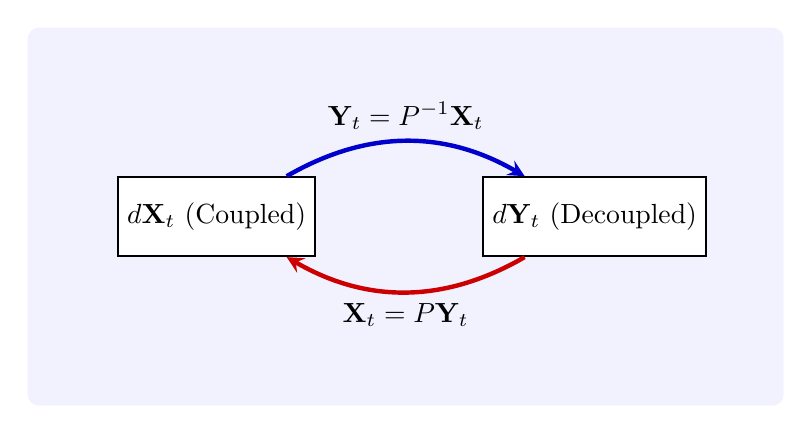
\begin{tikzpicture}[scale=1.2, >=stealth, thick]
    % Background
    \begin{scope}[on background layer]
        \fill[blue!5, rounded corners] (-2, -2) rectangle (6, 2);
    \end{scope}

    % Nodes
    \node[draw, rectangle, fill=white, text=black, minimum width=2.5cm, minimum height=1cm] (Coupled) at (0, 0) {$\displaystyle d\mathbf{X}_t \text{ (Coupled)}$};
    \node[draw, rectangle, fill=white, text=black, minimum width=2.5cm, minimum height=1cm] (Decoupled) at (4, 0) {$\displaystyle d\mathbf{Y}_t \text{ (Decoupled)}$};

    % Arrows
    \draw[->, ultra thick, blue!80!black] (Coupled) to[bend left=30] node[midway, above, text=black] {$\displaystyle \mathbf{Y}_t = P^{-1}\mathbf{X}_t$} (Decoupled);
    \draw[->, ultra thick, red!80!black] (Decoupled) to[bend left=30] node[midway, below, text=black] {$\displaystyle \mathbf{X}_t = P\mathbf{Y}_t$} (Coupled);
\end{tikzpicture}
\end{center}

\newpage
\section{Part 7: Common Variations and Untested Concepts}

\subsection{Defective Matrices and the Jordan Canonical Form}
The provided homework focuses exclusively on matrices that \textit{can} be diagonalized. However, a critical variation is dealing with \textbf{defective matrices}—matrices that do not have enough linearly independent eigenvectors to form a basis for $\R^n$.

\textbf{Example:} Consider $A = \begin{bmatrix} 1 & 1 \\ 0 & 1 \end{bmatrix}$. 
The characteristic equation is $(1-\lambda)^2 = 0$, so $\lambda = 1$ with algebraic multiplicity 2. 
To find the eigenvectors, we solve $(A - I)\mathbf{x} = \mathbf{0}$:
\[
\begin{bmatrix} 0 & 1 \\ 0 & 0 \end{bmatrix} \begin{bmatrix} x_1 \\ x_2 \end{bmatrix} = \begin{bmatrix} 0 \\ 0 \end{bmatrix}
\]
This implies $x_2 = 0$, and $x_1$ is free. The only eigenvector is $\mathbf{v}_1 = \begin{bmatrix} 1 \\ 0 \end{bmatrix}$. The geometric multiplicity is 1. Because $1 < 2$, we cannot form a $2 \times 2$ invertible matrix $P$. $A$ is defective and not diagonalizable. 

In advanced mathematics, when a matrix cannot be diagonalized, we instead reduce it to its \textbf{Jordan Canonical Form}, which is ``as close to diagonal as possible,'' placing 1s on the superdiagonal above the repeated eigenvalues.

\section{Part 8: Advanced Diagnostic Testing: ``Find the Flaw''}

\textit{Instructions: Act as the grader. Identify the subtle flaw in each solution, explain why it is incorrect in one sentence, and provide the correct final answer.}

\subsection{Problem 1}
\textbf{Task:} Diagonalize $A = \begin{bmatrix} 2 & 3 \\ 0 & 4 \end{bmatrix}$. \\
\textbf{Flawed Solution:} The matrix is triangular, so $\lambda_1 = 2, \lambda_2 = 4$. For $\lambda_1=2$, $\mathbf{v}_1 = \begin{bmatrix} 1 \\ 0 \end{bmatrix}$. For $\lambda_2=4$, $\mathbf{v}_2 = \begin{bmatrix} 3 \\ 2 \end{bmatrix}$. Therefore, $P = \begin{bmatrix} 3 & 1 \\ 2 & 0 \end{bmatrix}$ and $D = \begin{bmatrix} 2 & 0 \\ 0 & 4 \end{bmatrix}$. \\
\textbf{Flaw \& Correction:} The order of the eigenvectors in $P$ does not match the order of the eigenvalues in $D$; $\mathbf{v}_2$ is in the first column of $P$, but $\lambda_1$ is in the first column of $D$. \\
\textbf{Correct Answer:} $\displaystyle P = \begin{bmatrix} 1 & 3 \\ 0 & 2 \end{bmatrix}, \quad D = \begin{bmatrix} 2 & 0 \\ 0 & 4 \end{bmatrix}$

\subsection{Problem 2}
\textbf{Task:} Compute $A^3$ given $A = PDP^{-1}$. \\
\textbf{Flawed Solution:} Using the properties of matrix multiplication, we can distribute the exponent to get $A^3 = P^{-1}D^3P$. \\
\textbf{Flaw \& Correction:} Matrix multiplication is not commutative, and the correct telescoping cancellation yields $P$ on the left and $P^{-1}$ on the right, not the reverse. \\
\textbf{Correct Answer:} $\displaystyle A^3 = PD^3P^{-1}$

\subsection{Problem 3}
\textbf{Task:} Find the characteristic polynomial of $A = \begin{bmatrix} 1 & 2 \\ 2 & 1 \end{bmatrix}$. \\
\textbf{Flawed Solution:} $\det(A - \lambda I) = (1-\lambda)(1-\lambda) + (2)(2) = (1-\lambda)^2 + 4 = \lambda^2 - 2\lambda + 5$. \\
\textbf{Flaw \& Correction:} The determinant formula for a $2 \times 2$ matrix is $ad - bc$, so the student incorrectly added the off-diagonal product instead of subtracting it. \\
\textbf{Correct Answer:} $\displaystyle \det(A - \lambda I) = (1-\lambda)^2 - 4 = \lambda^2 - 2\lambda - 3$

\subsection{Problem 4}
\textbf{Task:} Is $A = \begin{bmatrix} 3 & 1 \\ 0 & 3 \end{bmatrix}$ diagonalizable? \\
\textbf{Flawed Solution:} Yes. The eigenvalue is $\lambda=3$ with an algebraic multiplicity of 2. We can simply use the eigenvector $\mathbf{v} = \begin{bmatrix} 1 \\ 0 \end{bmatrix}$ twice to form $P = \begin{bmatrix} 1 & 1 \\ 0 & 0 \end{bmatrix}$, making it diagonalizable. \\
\textbf{Flaw \& Correction:} The matrix $P$ must be invertible, which requires its columns to be linearly independent; repeating the same eigenvector makes $\det(P) = 0$. \\
\textbf{Correct Answer:} No, $A$ is defective and not diagonalizable.

\subsection{Problem 5}
\textbf{Task:} Find the inverse of $P = \begin{bmatrix} 2 & 4 \\ 1 & 3 \end{bmatrix}$ to compute $A = PDP^{-1}$. \\
\textbf{Flawed Solution:} Swapping the main diagonal and negating the off-diagonal gives $P^{-1} = \begin{bmatrix} 3 & -4 \\ -1 & 2 \end{bmatrix}$. \\
\textbf{Flaw \& Correction:} The student forgot to multiply the resulting matrix by the scalar $1/\det(P)$, which in this case is $1/(6-4) = 1/2$. \\
\textbf{Correct Answer:} $\displaystyle P^{-1} = \begin{bmatrix} 3/2 & -2 \\ -1/2 & 1 \end{bmatrix}$

\end{document}